\chapter{Final Project}

In this project we will configure a network combining the different technologies that we have learned along the course.
We will extend the topology in the routing assignment with wireless connectivity (WLAN) and security (Firewalls,IPSec) and traffic monitoring (Wireshark).

\section{Topology}

The topology that we will construct is presented in Fig. \ref{fig:final-topology}.
As in the routing assignments, each group will configure a part of the topology.
In this assignment, each group will take care of a router, a firewall, a switch, an access point and the necessary PCs.
This topology interconnects secured networks (behind a firewall) with another network that offers access to the Internet.
Each secured network needs at least a PC and an FTP server.

\begin{figure}
\centering
\ifpdf
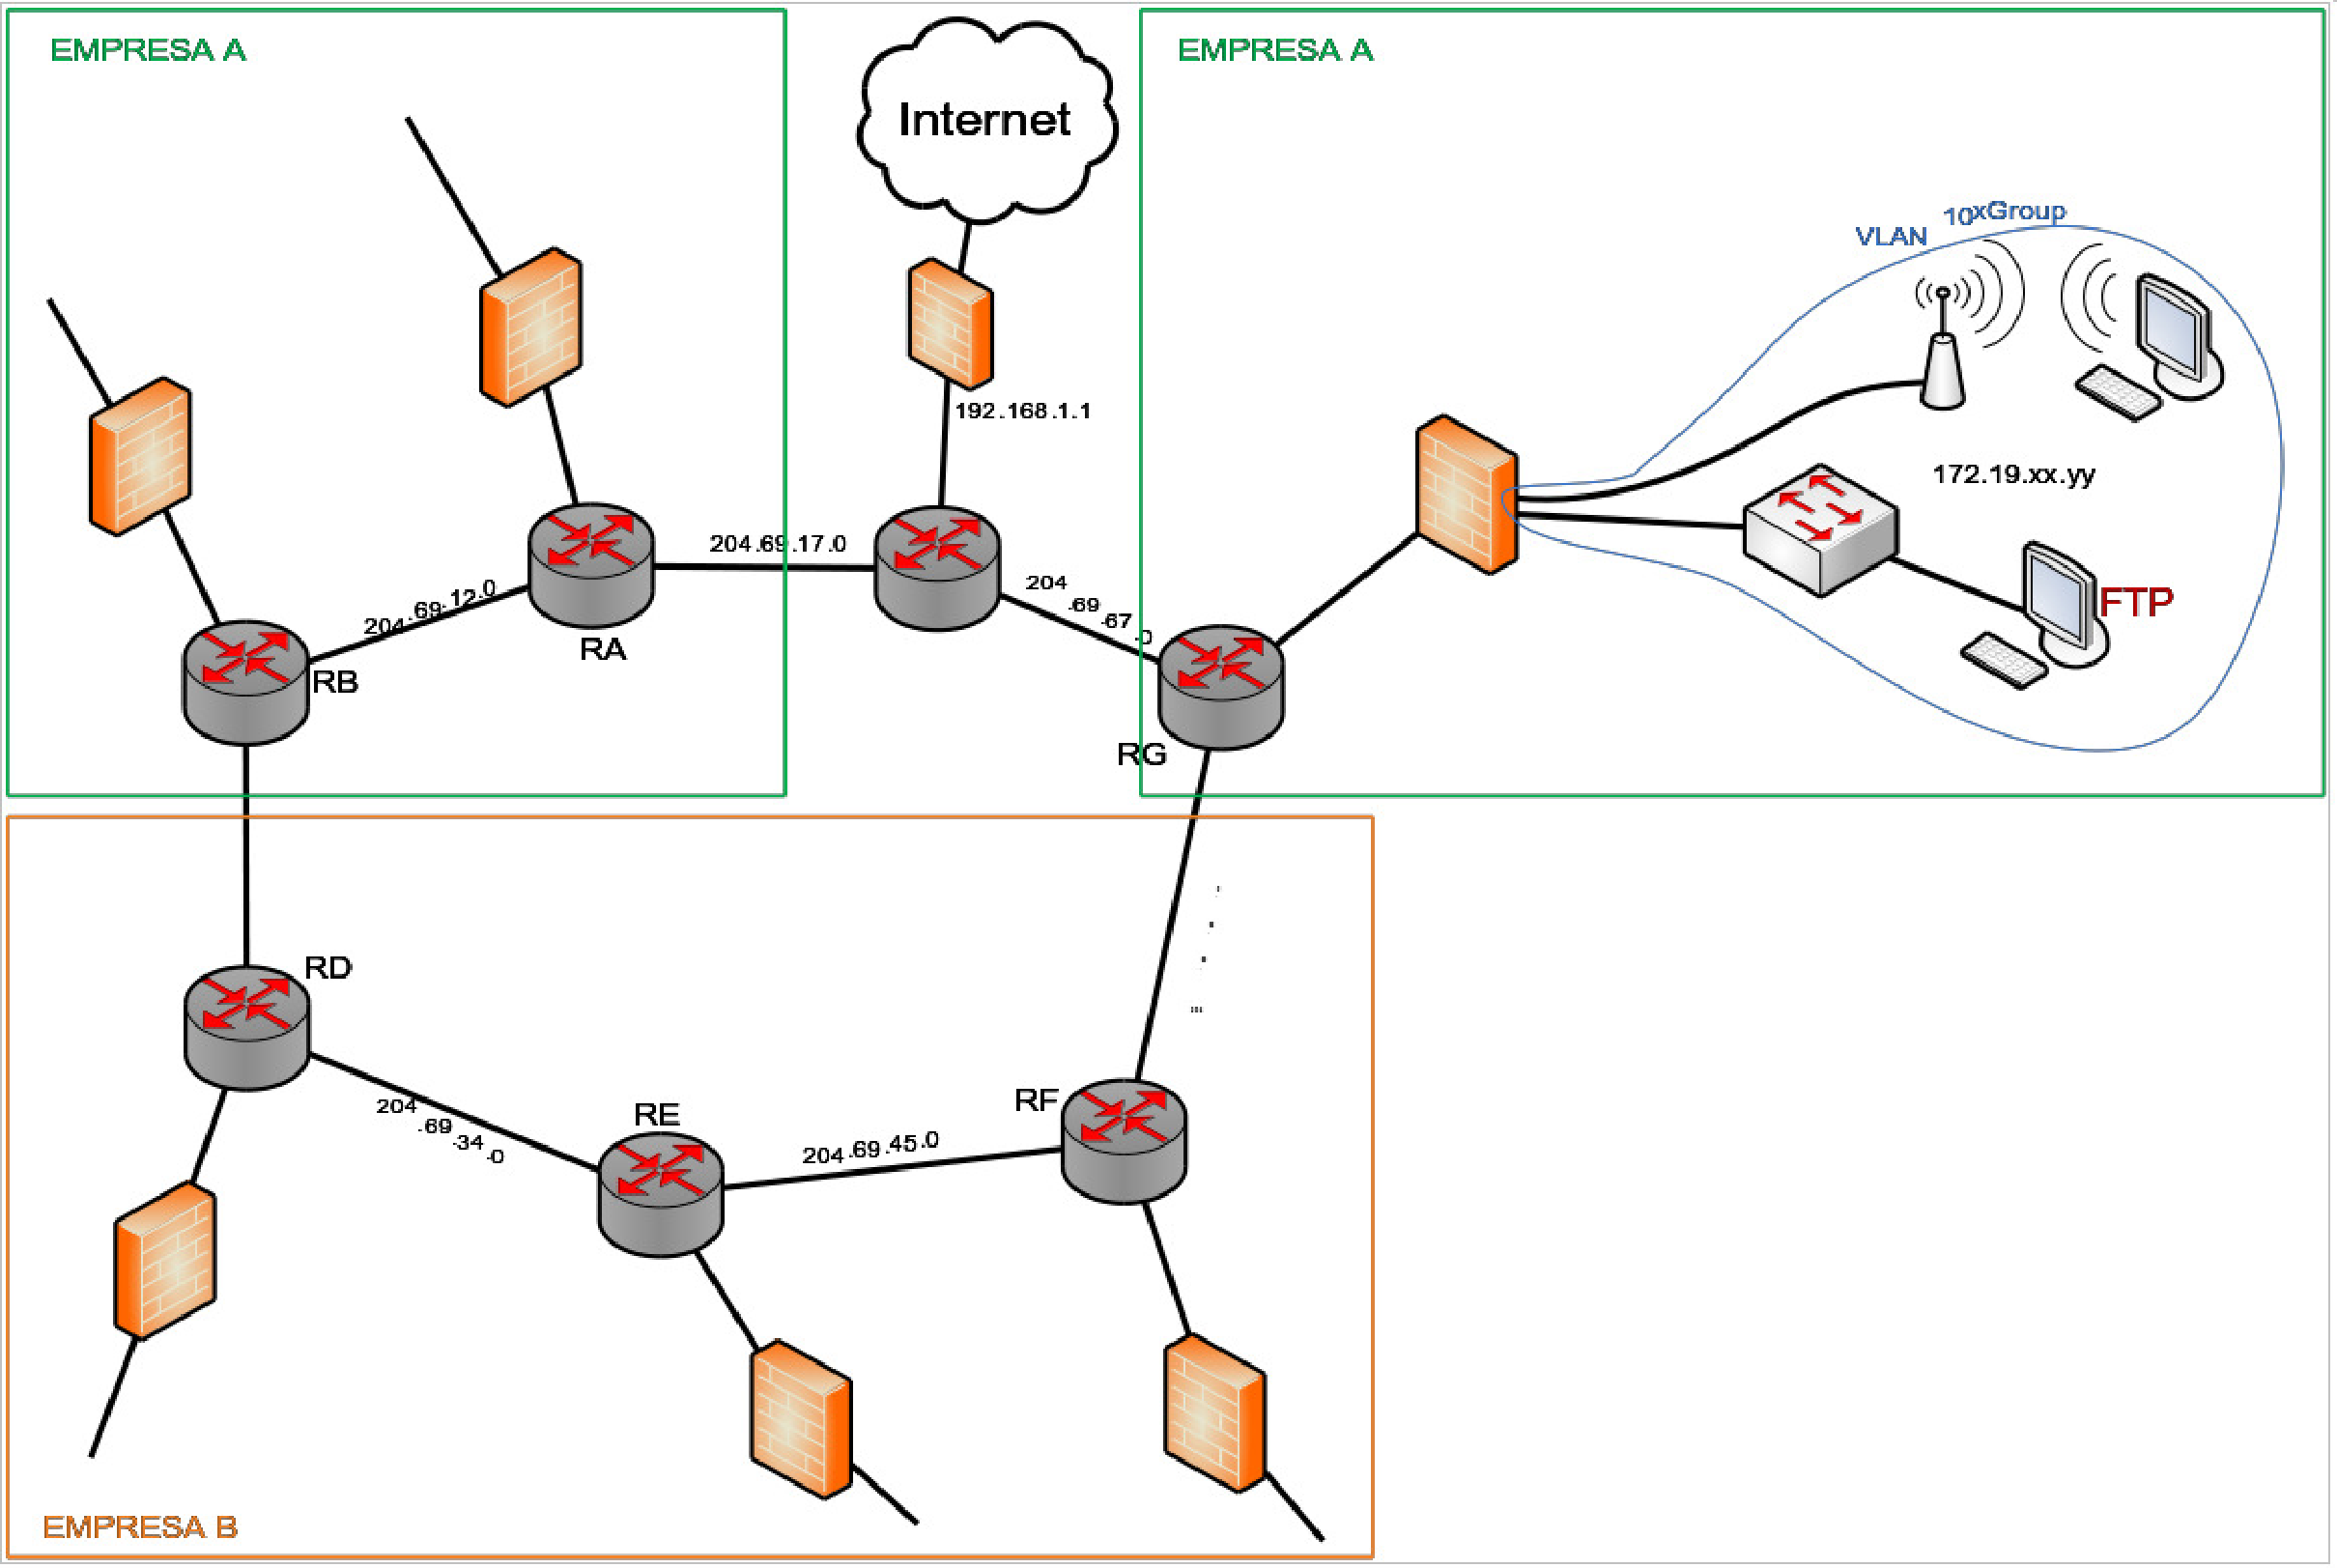
\includegraphics[width=0.9\linewidth]{Figures/final-topology.pdf}
\else
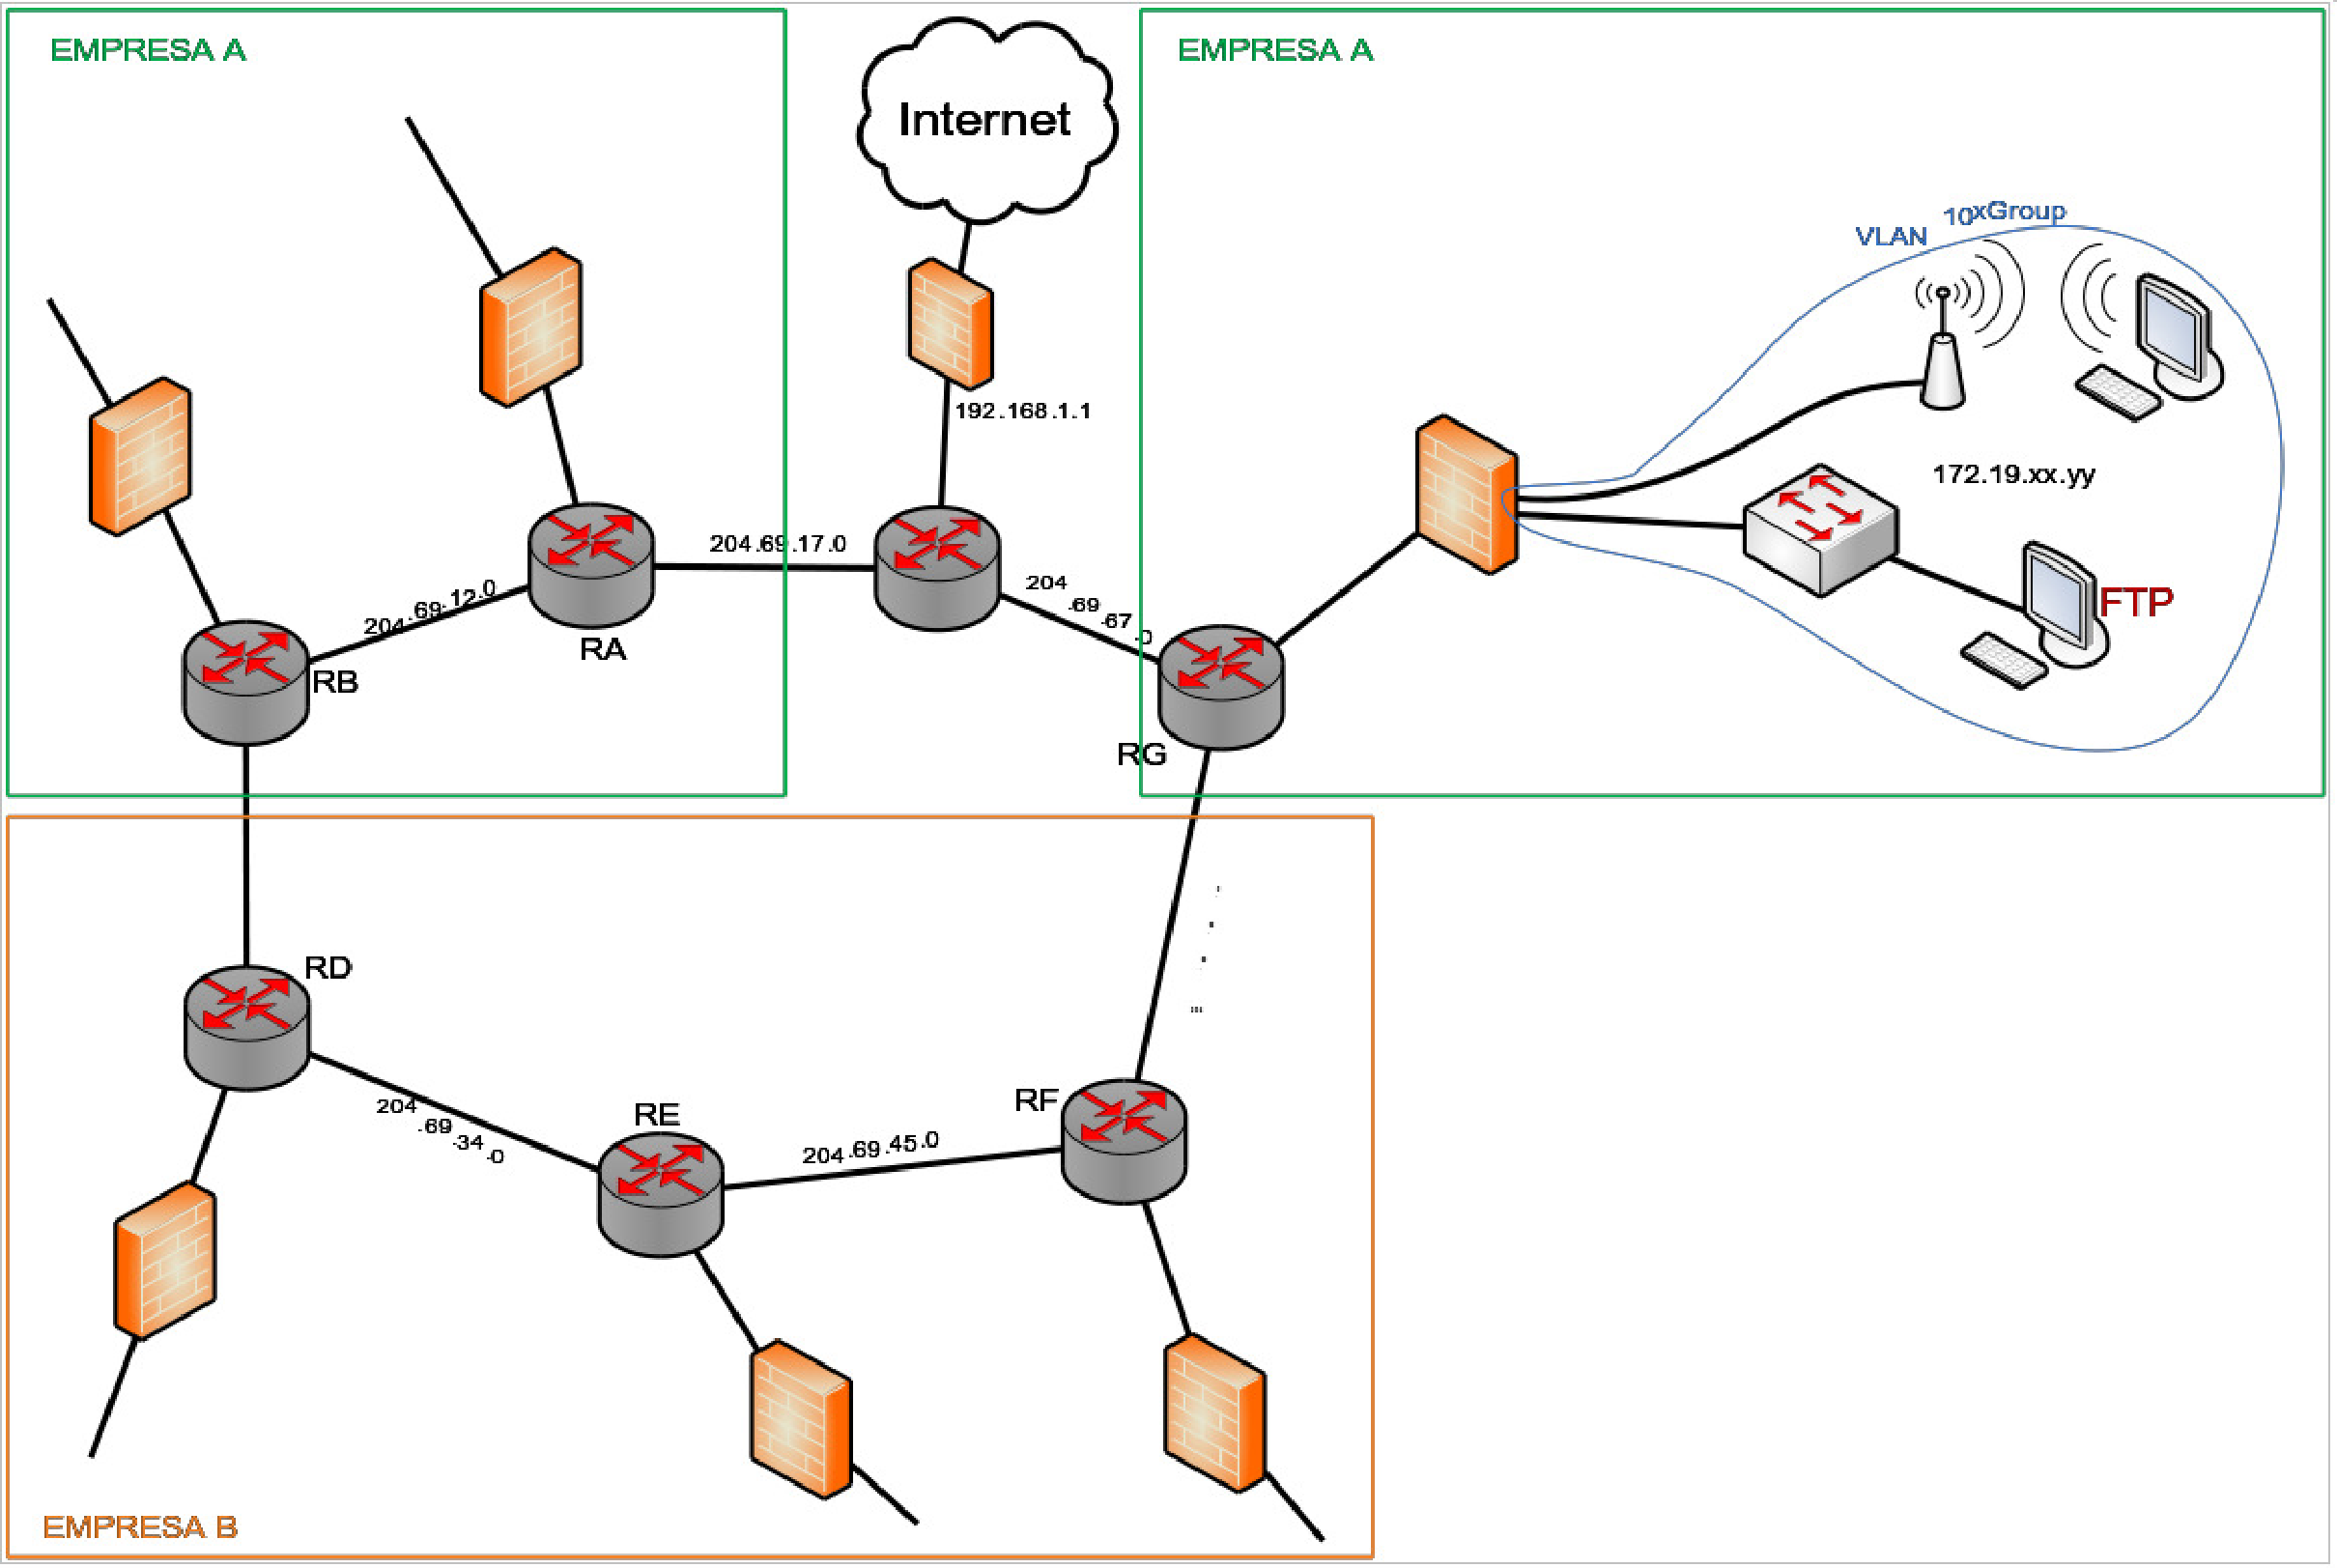
\includegraphics[width=0.9\linewidth]{Figures/final-topology.eps}
\fi
\caption{Topology of the final assignment}
\label{fig:final-topology}
\end{figure}

\section{Equipment and addresses}
The assignment of equipment and addresses to the groups is detailed in Table~\ref{tab:equipment-and-addresses}.
The switches are shared and the table specifies the ports for each group.
The IP addresses for WiFi devices, Ethernet devices, the FW interior interface and the public addresses are also included.

\begin{table}
\sffamily\small
\centering
\begin{tabular}{cccccccc}
\hline
Group & Router & Switch & Ports & IPs WiFi & IPs Eth & FWin & IPs public \\
\hline
1 & A & B & 1-6 & .80.1X/23 & .81.1X/23 & .80.1/23 & 201.69.10.0/24 \\
2 & B & B & 7-12 & .82.1X/23 & .83.1X/23 & .82.1/23 & 201.69.20.0/24 \\
3 & D & C & 1-6 & .84.1X/23 & .85.1X/23 & .84.1/23 & 201.69.30.0/24 \\
4 & E & C & 7-12 & .86.1X/23 & .87.1X/23 & .86.1/23 & 201.69.40.0/24 \\
5 & F & D & 1-6 & .88.1X/23 & .89.1X/23 & .88.1/23 & 201.69.50.0/24 \\
6 & G & D & 7-12 & .90.1X/23 & .91.1X/23 & .90.1/23 & 201.69.60.0/24 \\

\end{tabular}
\caption{Equipment and addresses}
\label{tab:equipment-and-addresses}
\end{table}


